\section{Schematics}

%TODO check this paragraph.  I have no idea what im talking about...
This section contains the system schematics. Figure~\ref{fig:systemSchematics} shows an updated version of the complete system schematic.  The circuit was divided in two two-layered PCBs which will be joined together by spacers and connectors. Figures~\ref{fig:firstBoard} and~\ref{fig:secondBoard} show the two levels of the designed PCB. 
\subsection{System Schematics}
\begin{figure}[H]
\centering
	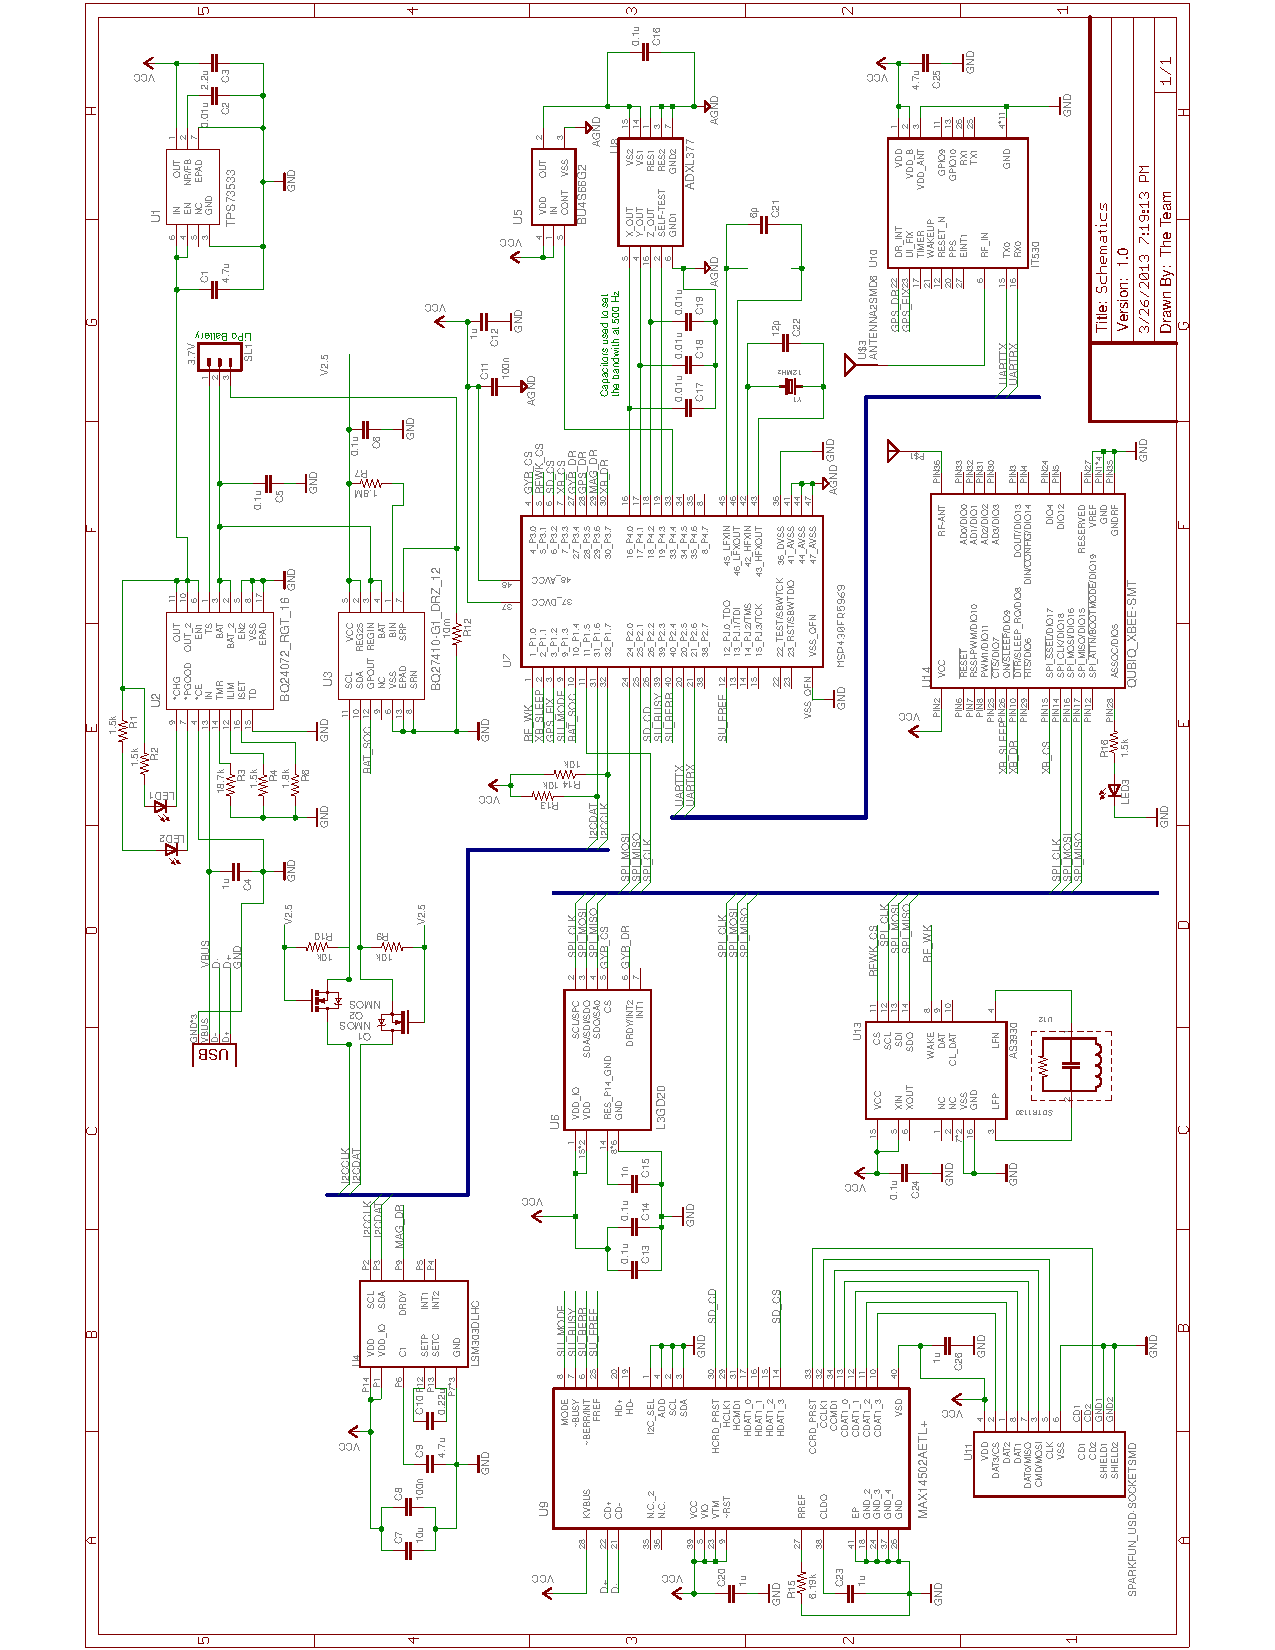
\includegraphics[width=\textwidth]{img/CompleteSchematics}
	\caption{System Schematic \label{fig:systemSchematics}}
\end{figure}

\begin{figure}[H]
\centering
	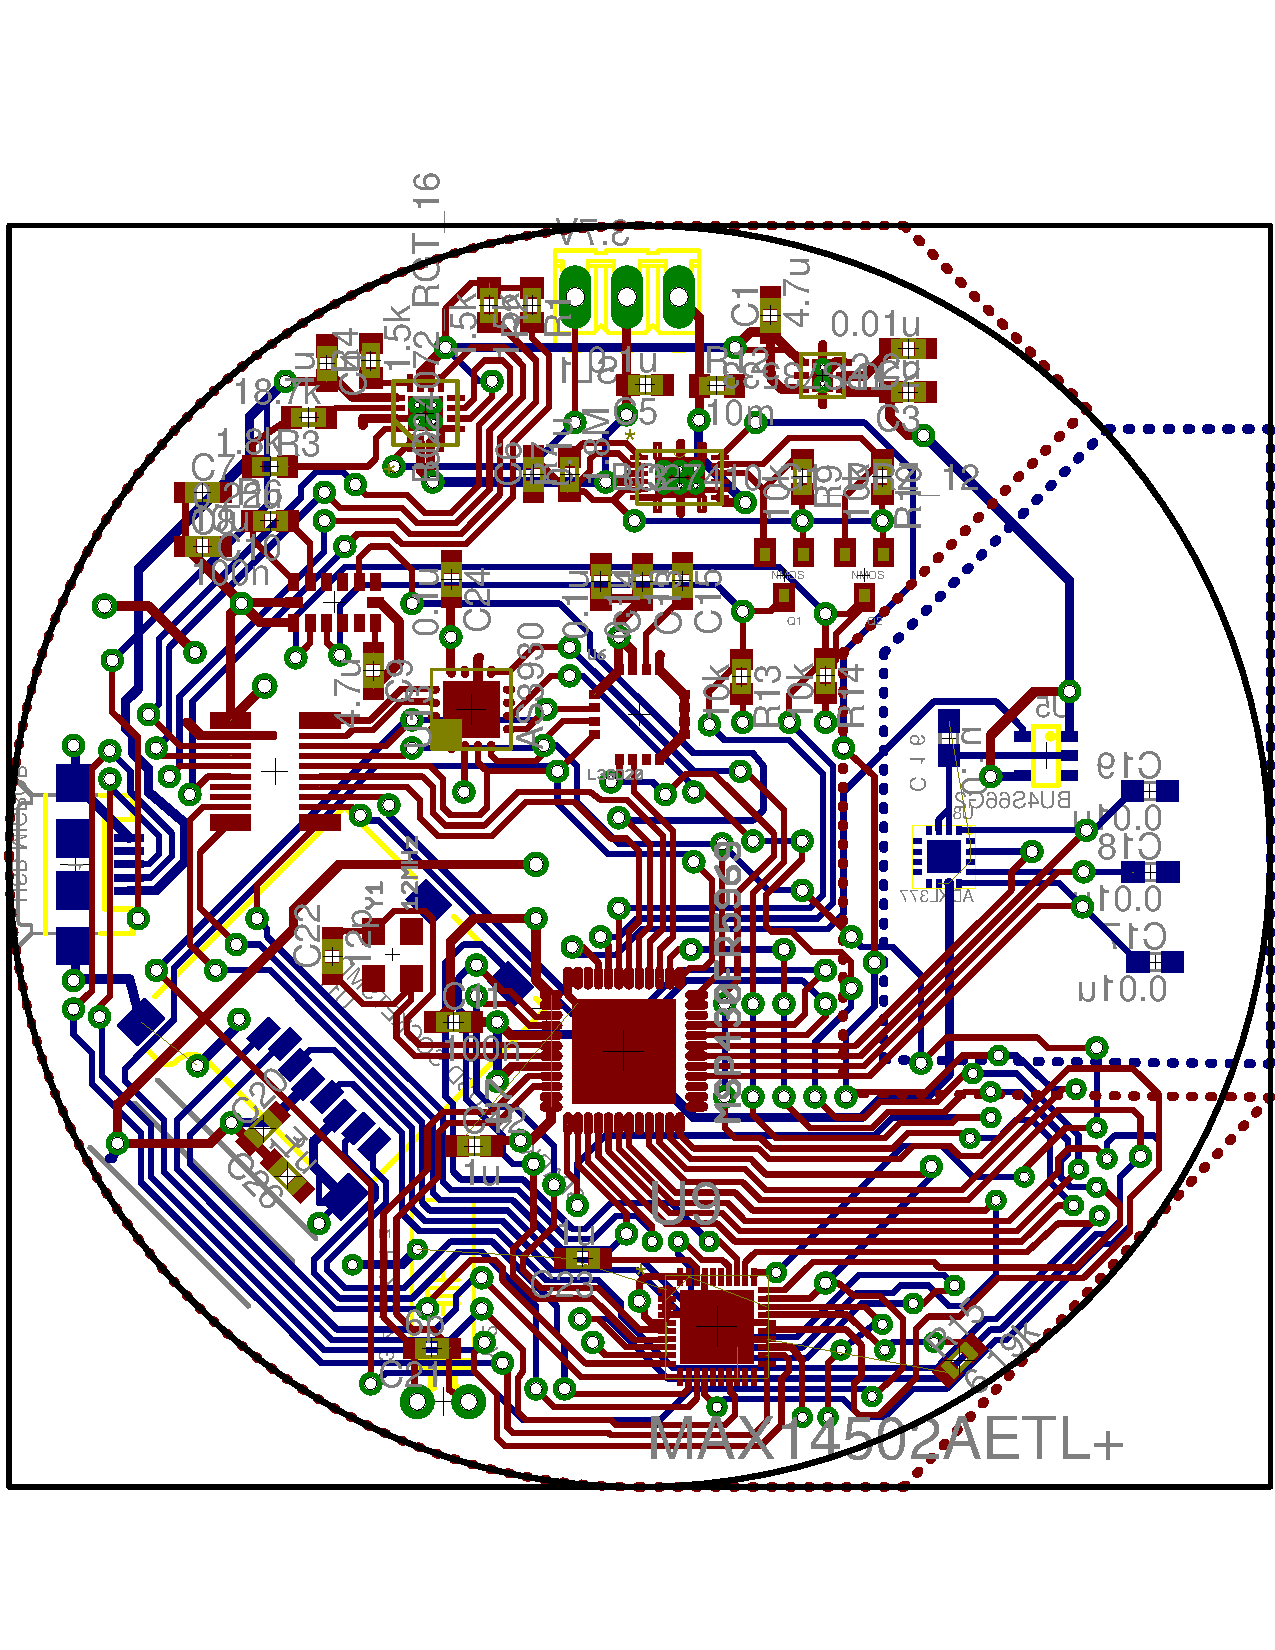
\includegraphics[width=\textwidth]{img/FirstLevelBoard}
	\caption{First Level Board Schematic \label{fig:firstBoard}}
\end{figure}

\begin{figure}[H]
\centering
	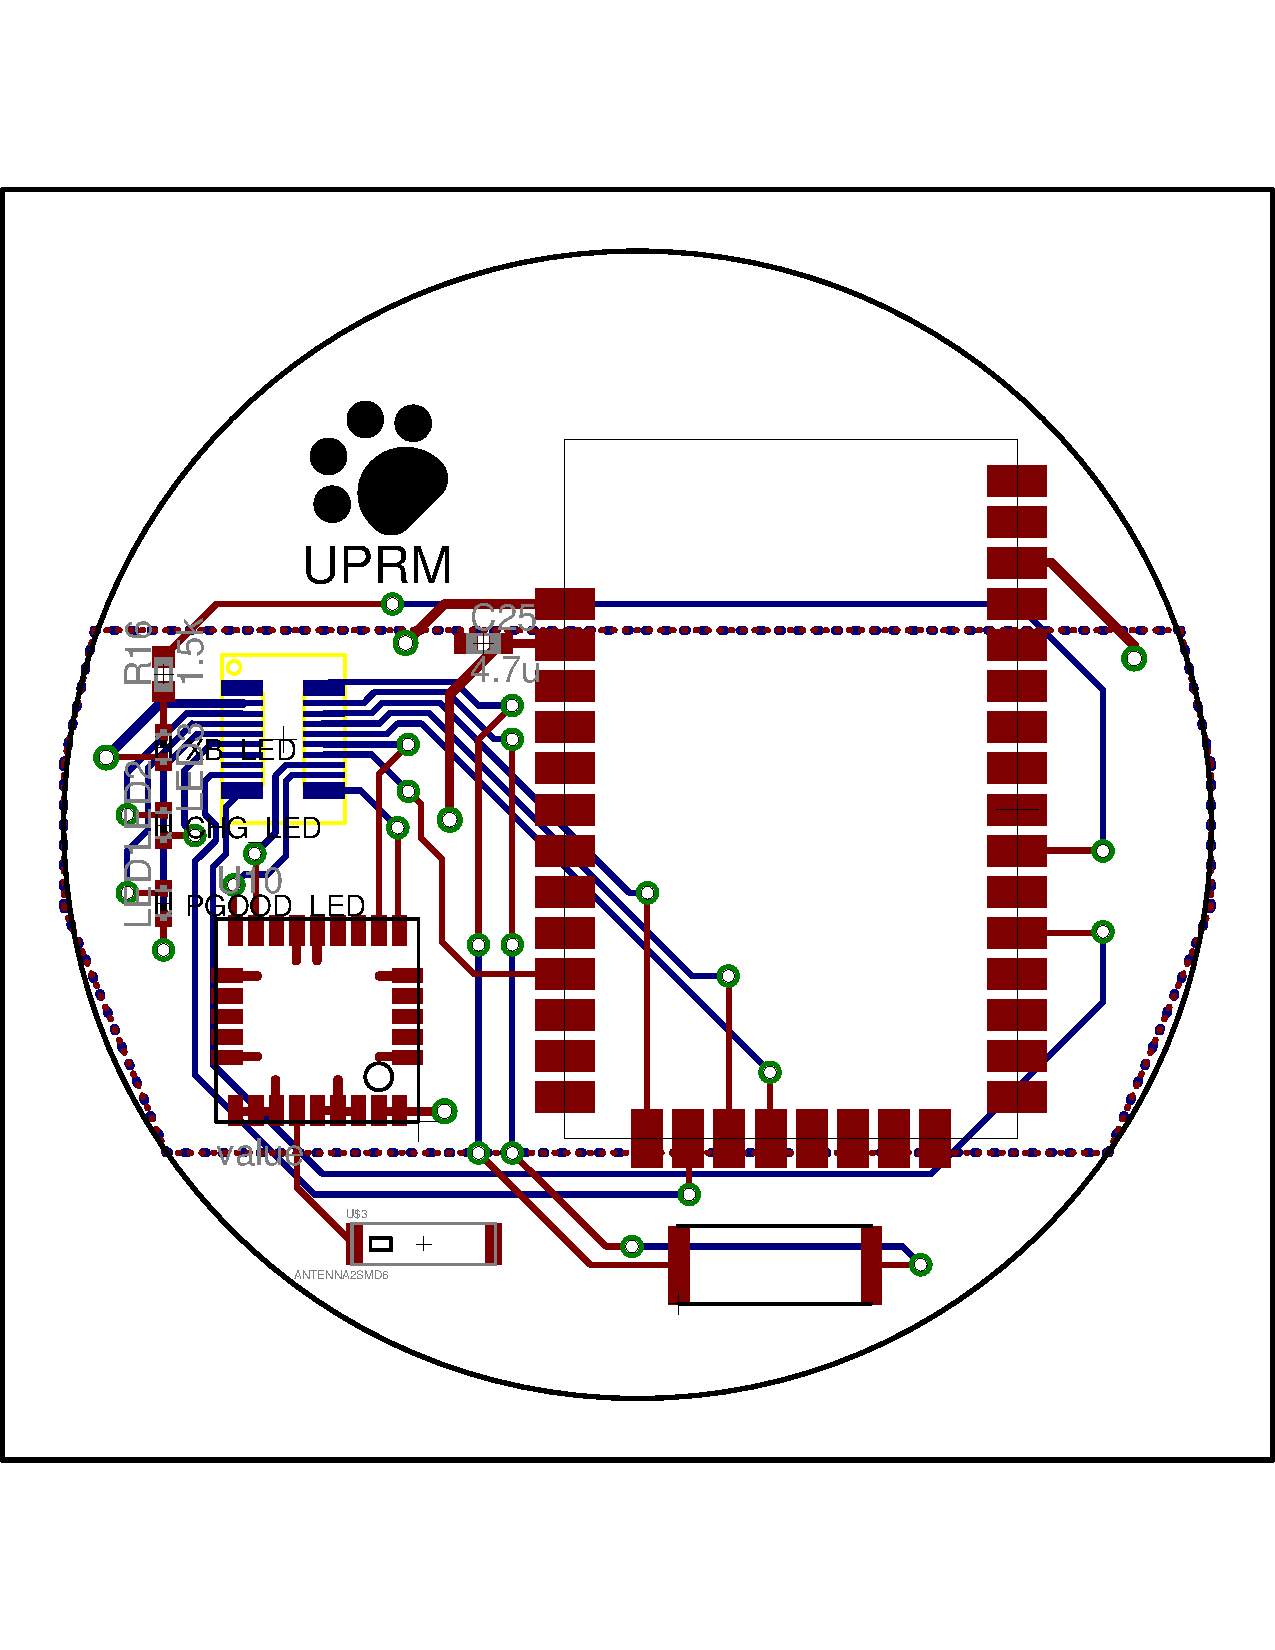
\includegraphics[width=\textwidth]{img/SecondLevelBoard}
	\caption{Second Level Board Schematic \label{fig:secondBoard}}
\end{figure}